\documentclass[12pt]{report}
\usepackage{geometry} \geometry{a4paper, top=20mm, left=20mm, right=20mm, bottom=20mm, headsep=10mm, footskip=12mm} 
\usepackage[T1]{fontenc}
\usepackage[utf8]{inputenc}
\usepackage[english]{babel}
\usepackage{amsmath}
\usepackage{amsfonts}
\usepackage{amssymb}

\usepackage[bookmarks=true]{hyperref}
\usepackage{bookmark}
\usepackage{graphicx}
\usepackage{csvsimple}
\usepackage {multicol}


\usepackage{color}
\definecolor{keyword}{rgb}{0.5,0,0.35}		% keywords
\definecolor{comments}{rgb}{0.2,0.5,0.25}	% comments
\definecolor{identifier}{rgb}{0.2,0.2,0.2}	% identifiers

\usepackage{listings}
\lstset{numbers = left, 		% Position of line numbers
	basicstyle = \ttfamily ,% Font type
	keywordstyle = \color{keyword},	% style for keywords
	commentstyle = \color{comments}, % style for comments
	stringstyle = \color{identifier}, 
	numberstyle = \small, 	% Font style of numbers
	numbersep = 7pt, 		% Space between line number and code
	breaklines = true,		% Automatic line breaking
	tabsize = 4,				% number of spaces for TAB
	language = Java,		% Used language
	frame = single
}


\begin{document}
\title{Stocks Specification}			% put title in brackets
\author{Jan Veen}
\maketitle				% create headings
\cleardoublepage
\pdfbookmark{\contentsname}{Contents}
\tableofcontents

\chapter{Data Model}

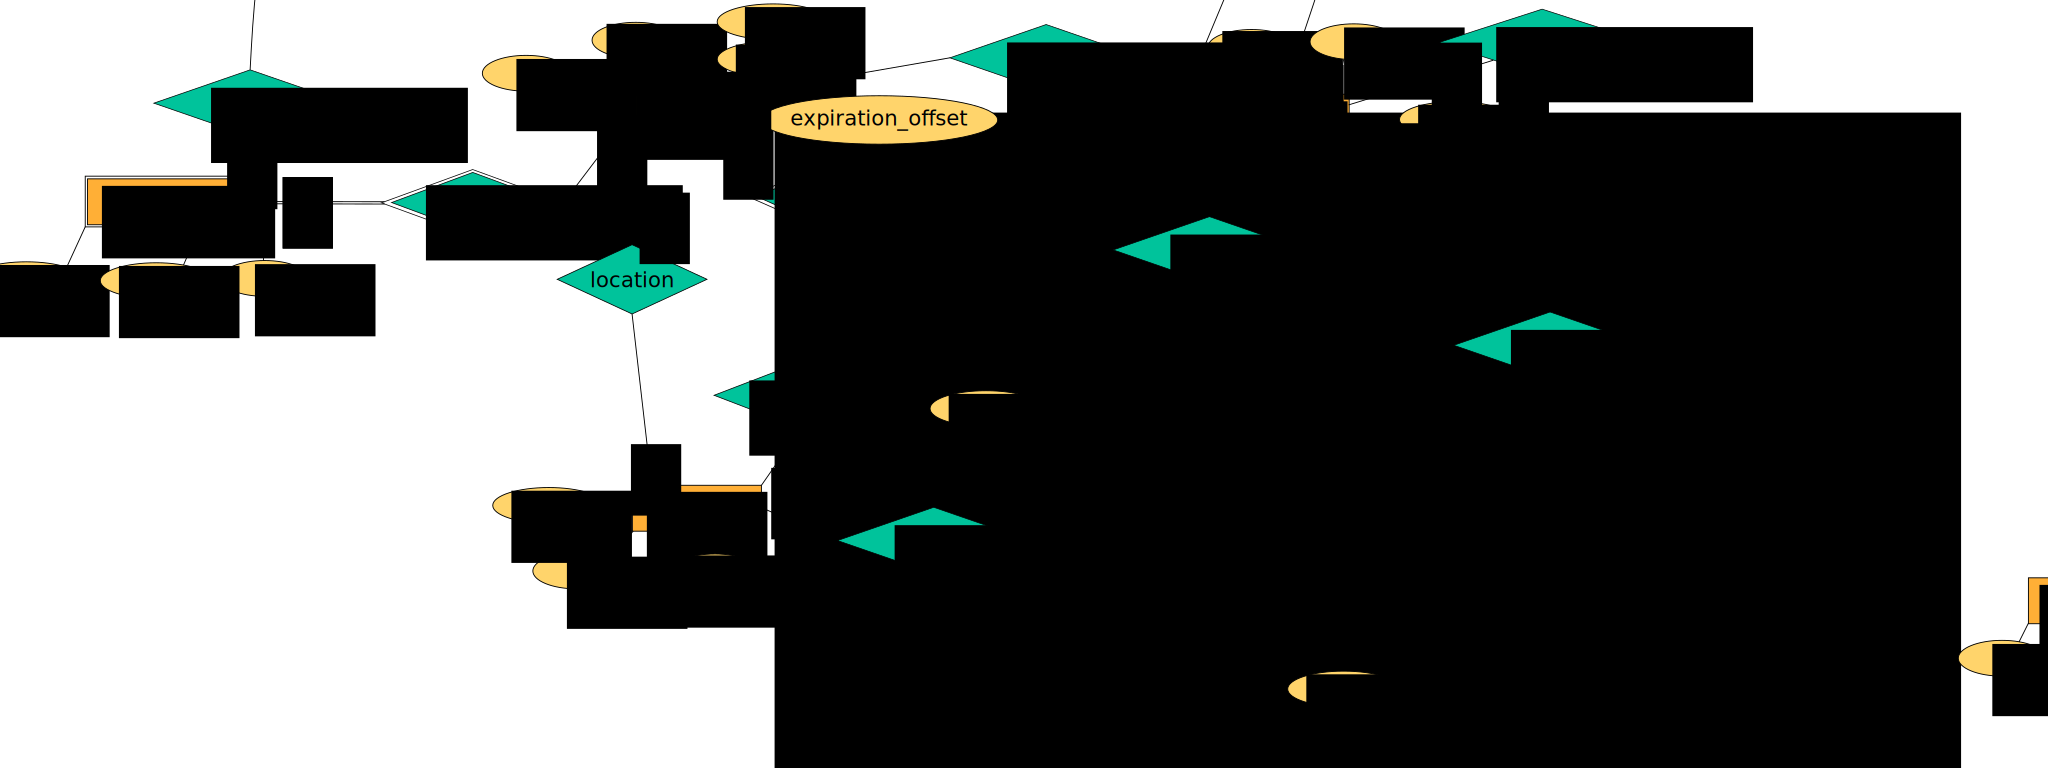
\includegraphics[width=\linewidth]{diagrams/ER-diagram.png}

\section{Date formats}
What date format is used in which part of the system:

\begin{tabular}{l l}
Location & Format \\\hline
Client code & Localtime \\\hline
Client database & UTC \\\hline
Network & UTC \\\hline
Server code & UTC \\\hline
Server database & UTC \\\hline
\end{tabular}

\chapter{Architecture}

\section{Client}

Here interesting use cases for clients interacting with the server
are described.

\subsection{Register New Data}

\includegraphics[width=\linewidth]{diagrams/put-data.png}

\subsection{Refresh client database}

\includegraphics[width=\linewidth]{diagrams/Refreshment.png}

\subsection{New user registration}

New users are always added by giving a ticket from an existing user. The details are outlined in the diagram. 

\includegraphics[width=\linewidth]{diagrams/new-user-registration.png}

\paragraph{Principal Names}
In the CSR the user stores the principals of his device. The values are formatted inside the Common Name attribute of the CSR. The pattern is \texttt{username\$user\_id\$ devicename\$device\_id}. So for the default test user this resolves to \texttt{John\$1\$Device\$1}. 
The principals are checked in the sentry part of the server before the certificate is signed. 

\paragraph{Client Verification}
Upon receiving a new device registration request, the sentry performs the following checks in order:
\begin{itemize}
\item Check if the ticket value presented by the client is found in the database
\item Check the device id associated with the ticket from the database with the device id from the CSR
\item Check if the remaining principals of the device match the CSR
\item Check if the ticket has expired
\end{itemize}
If all the checks succeed the sentry has the CSR signed by the CA and returns it to the client. 

\paragraph{QR Code Tickets}
For mobile clients it is more convenient to pass the ticket as QR code. To generate this QR code the content of the ticket has to be
entered text into the QR code. The order of the values is the same as in the diagram description. 

\subsection{Device removal}

\includegraphics[width=\linewidth]{diagrams/remove-device.png}

\chapter{REST API}

List of all available endpoints, methods, their parameters and result types. 
Only \texttt{v2} endpoints are listed as their usage is strongly encouraged.

Response type schemas are indicated in a pseudo JSON notation. The anonymous
object ontop of each description is the root object. Any further types used
in that root object are described in \ref{common-data-structures} or directly
under the root object.

\section{Common Data Types}\label{common-data-structures}

\subsection{Versions}

Each entity in the system has a version which is incremented each
time the entity is edited. This means all modifying operations have
to pass the correct version of the entity to edit. If the version does
not match an error is returned using status codes, see \ref{status-codes}
for a list of status codes to support.

\subsection{Status codes}\label{status-codes}

Numbers reporting the result status of a request. The API refers to this
via the \texttt{StatusCode} type.

\begin{itemize}
\item 0: Success
\item 1: General error
\item 2: Not found
\item 3: Invalid data version
\item 4: Foreign key constraint violation
\item 5: Database unreachable
\item 6: Access denied
\item 7: Invalid argument
\item 8: Certificate authority unreachable
\end{itemize}

\subsection{Timestamps}

The timestamp format used is \texttt{yyyy.MM.dd-HH:mm:ss.SSS-Z}. Refer to\\
https://docs.oracle.com/javase/8/docs/api/java/time/format/DateTimeFormatter.html
for semantics. The timestamps are passed as strings.

\subsection{Response}
Most calls only return a basic response with a status code. They have the
following shape:
\begin{lstlisting}
Response {
    status: StatusCode
}
\end{lstlisting}

\section{Sentry}

Endpoints listed here are only reachable via the sentry port. \\\\
\texttt{POST /v2/auth/newuser}: Register new device\\
Form parameters:
\begin{itemize}
\item \texttt{device: int} The id of the device which wants to register
\item \texttt{token: String} The token generated when creating the new device
\item \texttt{csr: String} The PEM X.509 Certificate Signing Request generated by the device
\end{itemize}
Result: \texttt{application/json}
\begin{lstlisting}
{
    status: StatusCode
    data: String // PEM X.509 certificate signed by the stocks CA
}
\end{lstlisting}

\section{Server}

\subsection{Updates}

\texttt{GET /v2/update}: Get change timestamps of entities\\
No parameters\\
Result: \texttt{application/json}
\begin{lstlisting}
{
    status: StatusCode
    data: List<Update>
}

Update {
    table: String
    lastUpdate: Timestamp // yyyy.MM.dd-HH:mm:ss.SSS-Z
}
\end{lstlisting}

\subsection{Users}

\texttt{GET /v2/user}: Get all users in the system\\
No parameters\\
Result: \texttt{application/json}
\begin{lstlisting}
{
    status: StatusCode
    data: List<User>
}

User {
    id: int
    version: int
    name: String
}
\end{lstlisting}\vspace{7mm}
\texttt{PUT /v2/user}: Add a new user into the system\\
Query parameters:
\begin{itemize}
\item \texttt{name: String} The name of the new user
\end{itemize}
Result: \texttt{application/json}, \texttt{Response}\vspace{7mm}\\
\texttt{DELETE /v2/user}: Delete a user and all their devices from the system.
The calling user is set on all food items registered by the deleted devices.
Access to the system is revoked for all devices of the deleted user.\\
Query parameters:
\begin{itemize}
\item \texttt{id: int} The ID of the user to delete
\item \texttt{version: int} The current version of the user to be deleted
\end{itemize}
Result: \texttt{application/json}, \texttt{Response}

\subsection{Devices}

\texttt{PUT /v2/device}: Create a new device in the system. This query yields
both the ID of the newly created device as well as the ticket token needed to
register at the sentry.\\
Query parameters:
\begin{itemize}
\item \texttt{name: String} The name of the new device
\item \texttt{belongsTo: int} The user ID of the user to whom the device belongs
\end{itemize}
Result: \texttt{application/json}
\begin{lstlisting}
{
    status: StatusCode
    data: ClientTicket
}

ClientTicket {
    deviceId: int    // Device ID
    ticket: String
}
\end{lstlisting}\vspace{7mm}
\texttt{GET /v2/device}: Get all devices in the system\\
No parameters\\
Result: \texttt{application/json}
\begin{lstlisting}
{
    status: StatusCode
    data: List<Device>
}

Device {
    id: int
    version: int
    name: String
    userId: int   // User ID
}
\end{lstlisting}\vspace{7mm}
\texttt{DELETE /v2/device}: Delete a device from the system.
Access to the system is revoked for that device. The caller
is set on all food items that have been registered by the deleted
device.\\
Query parameters:
\begin{itemize}
\item \texttt{id: int}: The ID of the device to be deleted
\item \texttt{version: int}: The version of the device to be deleted
\end{itemize}
Result: \texttt{application/json}, \texttt{Response}

\subsection{Food}

\texttt{PUT /v2/food}: Add a food type to the system.\\
Query parameters:
\begin{itemize}
\item \texttt{name: String}: The name of the new food type
\end{itemize}
Result: \texttt{application/json}, \texttt{Response}\vspace{7mm}\\
\texttt{GET /v2/food}: Get all food types in the system.
No parameters.\\
Result: \texttt{application/json}
\begin{lstlisting}
{
    status: StatusCode
    data: List<Food>
}

Food {
    id: int
    version: int
    name: String
}
\end{lstlisting}\vspace{7mm}
\texttt{PUT /v2/food/rename}: Rename an existing food type.\\
Query parameters:
\begin{itemize}
\item \texttt{id: int}: The ID of the food type to rename
\item \texttt{version: int}: The version of the food type
\item \texttt{new: String}: The name to which the food type shall be renamed
\end{itemize}
Result: \texttt{application/json}, \texttt{Response}\vspace{7mm}\\
\texttt{DELETE /v2/food}: Delete a food type. This also deletes all food
items of this type.\\
Query parameters:
\begin{itemize}
\item \texttt{id: int} The ID of the food type to delete
\item \texttt{version: int} The version of the food type to delete
\end{itemize}
Result: \texttt{application/json}, \texttt{Response}

\subsection{Locations}

\texttt{PUT /v2/location}: Add a new location into the system.\\
Query parameters:
\begin{itemize}
\item \texttt{name: String}: The name of the new location
\end{itemize}
Result: \texttt{application/json}, \texttt{Response}\vspace{7mm}\\
\texttt{GET /v2/location}: Get the locations of the system.\\
No parameters.\\
Result: \texttt{application/json}
\begin{lstlisting}
{
    status: StatusCode
    data: List<Location>
}

Location {
    id: int
    version: int
    name: String
}
\end{lstlisting}\vspace{7mm}
\texttt{PUT /v2/location/rename}: Rename an existing location.\\
Query parameters:
\begin{itemize}
\item \texttt{id: int}: The ID of the location to rename
\item \texttt{version: int}: The version to rename
\item \texttt{new: String}: The new name of the location
\end{itemize}
Result: \texttt{application/json}, \texttt{Response}\vspace{7mm}\\
\texttt{DELETE /v2/location}: Delete a location. Deleting a location containing
food items is restricted by default, raising status code 4. When setting the
cascade flag, the items stored in that location will be deleted as well.\\
Query parameters:
\begin{itemize}
\item \texttt{id: int}: The ID of the location to rename
\item \texttt{version: int}: The version to rename
\item \texttt{cascade: int}: Set to 1 to delete all food items contained
in the location as well.
\end{itemize}
Result: \texttt{application/json}, \texttt{Response}\vspace{7mm}\\

\subsection{EAN Numbers}

\texttt{PUT /v2/ean}: Add a new EAN code to the system.\\
Query parameters:
\begin{itemize}
\item \texttt{code: String}: The EAN code to register
\item \texttt{identifies: int}: The Food type ID the code shall be associated
with.
\end{itemize}
Result: \texttt{application/json}, \texttt{Response}\vspace{7mm}\\
\texttt{GET /v2/ean}: Get the EAN codes of the system.\\
No parameters
Result: \texttt{application/json}
\begin{lstlisting}
{
    status: StatusCode
    data: List<EanNumber>
}

EanNumber {
    id: int
    version: int
    eanCode: String
    identifiesFood: int	    // Food ID
}
\end{lstlisting}
\texttt{DELETE /v2/ean}: Delete an EAN Code from the system.\\
Query parameters:
\begin{itemize}
\item \texttt{id: int}: The ID of the EAN code to delete
\item \texttt{version: int}: The version of the EAN code to delete
\end{itemize}
Result: \texttt{application/json}, \texttt{Response}\vspace{7mm}\\

\subsection{Food items}

\texttt{PUT /v2/fooditem}: Put a new food item into the system.\\
Query parameters:
\begin{itemize}
\item \texttt{eatByDate: Timestamp}: The date by which the item should be
consumed.
\item \texttt{storedIn: int}: The ID of the location to store the item in
\item \texttt{ofType: int}: The ID of the food type to which the item belongs
\end{itemize}
Result: \texttt{application/json}, \texttt{Response}\vspace{7mm}\\
\texttt{GET /v2/fooditem}: Get all the food items in the system\\
No parameters\\
Result: \texttt{application/json}
\begin{lstlisting}
{
    status: StatusCode
    data: List<FoodItem>
}

FoodItem {
	id: int
	version: int
	eatByDate: Timestamp
	storedIn: int         // Location ID
	ofType: int           // Food ID
	registers: int        // Device ID
	buys: int             // User ID
}
\end{lstlisting}
\texttt{PUT /v2/fooditem/edit}: Edit an existing food item.\\
Query parameters:
\begin{itemize}
\item \texttt{id: int}: The ID of the food item to edit
\item \texttt{version: int}: The version of the food item to edit
\item \texttt{eatByDate: Timestamp}: The new date by which the item should be
consumed
\item \texttt{storedIn: int}: The ID of the new location to store the item in
\end{itemize}
Result: \texttt{application/json}, \texttt{Response}\vspace{7mm}\\

\texttt{DELETE /v2/fooditem}: Delete a food item.\\
Query parameters:
\begin{itemize}
\item \texttt{id: int}: The ID of the food item to delete
\item \texttt{version: int}: The version of the food item to delete
\end{itemize}
Result: \texttt{application/json}, \texttt{Response}\vspace{7mm}\\

\end{document}
